\documentclass[pdflatex,iicol,sn-mathphys-num]{sn-jnl}

\usepackage{graphicx}
\usepackage{multirow}
\usepackage{amsmath,amssymb,amsfonts}
\usepackage{amsthm}
\usepackage[title]{appendix}
\usepackage{xcolor}
\usepackage{booktabs}
\usepackage{algorithm}
\usepackage{algorithmicx}
\usepackage{algpseudocode}
\usepackage{subcaption}
\usepackage{array}
\usepackage{url}
\usepackage{tikz}
\usetikzlibrary{arrows.meta,shapes.geometric}

\newcommand{\method}{\textsc{FuseTune}}
\newcommand{\codeid}{\texttt{fusetune}}
\newcommand{\loss}{\mathcal{L}}
\def\UrlBreaks{\do\/\do-\do\_}

\usepackage{hyperref}
\pdfstringdefDisableCommands{%
  \def\textsc#1{#1}%
  \def\texttt#1{#1}%
  \def\method{FuseTune}%
  \def\codeid{fusetune}%
  \def\ell{l}%
}

\raggedbottom

\begin{document}

\title[\method{} for Fused Regression]{\method{}: Low-Budget Hyperparameter Tuning for Fused Regression}

%%% TODO: Replace placeholder author names, emails, ORCIDs, and affiliation before submission.
\author*[1]{\fnm{First} \sur{Author}}\email{first.author@example.com}
\equalcont{These authors contributed equally to this work.}
\author[1]{\fnm{Second} \sur{Author}}\email{second.author@example.com}

\affil*[1]{\orgdiv{Department}, \orgname{Institution}, \orgaddress{\street{Street Address}, \city{City}, \postcode{00000}, \state{State}, \country{Country}}}

\abstract{
Fused regression models rely on two coupled hyperparameters: a sparsity penalty and a fusion penalty. In practice these hyperparameters are often tuned by exhaustive grids or warm-start heuristics, even though each cross-validation evaluation can be expensive and the validation surface can be noisy, solver-dependent, and strongly dataset-dependent. We present \method{}, a low-budget tuning procedure for fused regression that searches in log-parameter space and adapts its strategy to the solver. For the \(\ell_1\) fused solver, \method{} uses a nonmonotone axis-aligned direct search. For the \(\ell_2\) fused solver, it uses a redesigned \texttt{glmnet}-seeded hybrid search that screens a small set of candidates before conditional local refinement. Across nine real \(\ell_1\) datasets, \method{} is faster than \texttt{glmnet}-seeded on all datasets while matching or improving test RMSE on seven. On nine real \(\ell_2\) datasets, the redesigned \method{} is faster than \texttt{glmnet}-seeded on eight datasets and nearly ties its mean test RMSE while using less than half the average number of validation evaluations. Synthetic regime studies show that \method{} is the strongest efficiency method for \(\ell_1\), and a credible low-budget alternative for \(\ell_2\), especially in regimes where fusion is helpful. The contribution is practical rather than theoretical: we do not claim a new optimization class, but a reproducible, solver-aware tuning strategy for fused regression.
}

\keywords{fused regression, hyperparameter tuning, derivative-free optimization, cross-validation, regularization}

\maketitle

\section{Introduction}
Fused regression is attractive when related groups may share coefficient structure without being identical. A fused model allows each group to retain its own coefficients while borrowing strength through a penalty on inter-group differences. This idea is useful when partial similarity is plausible but complete pooling is too strong. The practical difficulty is that fused regression introduces at least two interacting hyperparameters: a sparsity penalty \(\lambda\) and a fusion penalty \(\gamma\). Their joint choice is usually made by cross-validation, yet cross-validation is exactly where the computational bottleneck appears.

The tuning problem is awkward for three reasons. First, each objective evaluation is expensive because it nests model fitting inside repeated train-validation splits. Second, the cross-validation surface can be non-smooth or effectively noisy because folds, group structure, and solver failures all affect the observed score. Third, the preferred region of \((\lambda,\gamma)\) is not stable across datasets or even across solver families. In some datasets fusion is clearly helpful; in others the best choice is close to no fusion at all. A useful tuner therefore needs to be cheap, robust, and cautious about spending evaluation budget where the surface gives little return.

This paper studies that tuning problem empirically and proposes \method{}, a solver-aware low-budget tuner for fused regression. The method is deliberately modest. For the \(\ell_1\) fused solver it performs a nonmonotone axis-aligned direct search in log-parameter space. For the \(\ell_2\) fused solver it uses a different design: a \texttt{glmnet}-seeded hybrid search that screens a few candidates, refines \(\gamma\) first, and only touches \(\lambda\) locally when the screening stage justifies it. The central claim is not that \method{} defines a new optimization class. The claim is that fused-regression tuning benefits from a small, solver-aware search procedure that spends the validation budget where it matters.

Our main empirical findings are straightforward. On the retained real-data \(\ell_1\) suite, \method{} is faster than \texttt{glmnet}-seeded on all nine datasets and no worse in test RMSE on seven. On the retained real-data \(\ell_2\) suite, the redesigned \method{} is faster than \texttt{glmnet}-seeded on eight of nine datasets, has lower mean test RMSE by a negligible margin, and uses roughly \(9.6\) validation evaluations on average versus \(20.4\) for \texttt{glmnet}-seeded. On synthetic regimes, \method{} is the strongest efficiency method for \(\ell_1\), and after the \(\ell_2\) redesign it becomes a credible low-budget alternative there as well, although not the raw-RMSE winner on average.

In summary, the contributions of this paper are:
\begin{itemize}
\item A solver-aware, low-budget tuning procedure for fused regression that adapts its outer search to the inner solver: nonmonotone axis-aligned direct search for the \(\ell_1\) solver and a \texttt{glmnet}-seeded hybrid for the \(\ell_2\) solver.
\item A normalized gain-per-second efficiency metric that makes the accuracy--budget trade-off explicit across datasets and methods.
\item An empirical benchmark on nine real datasets per solver and 30~synthetic regimes showing that \method{} is consistently faster than the warm-start baseline while retaining nearly all predictive performance.
\end{itemize}

The paper is organized as follows. Section~\ref{sec:related} positions the work relative to fused penalties and derivative-free search. Section~\ref{sec:method} presents the problem setup, \method{}, and the efficiency metric used in the comparisons. Section~\ref{sec:design} summarizes the experimental design. Section~\ref{sec:results} presents the real-data, synthetic, and surface-diagnostic results. Section~\ref{sec:discussion} closes with practical interpretation and limitations.

\section{Related Work}\label{sec:related}
Classical regularized regression starts with the lasso and extends naturally to nonconvex, grouped, and mixed penalties \cite{tibshirani1996lasso,fan2001scad,zou2005elastic,yuan2006group,zou2006adaptive,simon2013sparsegroup}. These papers matter here for two reasons. First, they establish the statistical motivation for imposing structured shrinkage rather than treating each coefficient independently. Second, they show that once a model carries multiple regularization terms, the outer hyperparameter search becomes a central practical problem rather than a minor implementation detail.

Fusion penalties and related coefficient-clustering formulations form the immediate statistical background. The fused lasso itself couples sparsity and local smoothness \cite{tibshirani2005fused}, while later work developed pathwise coordinate methods, specialized path algorithms, generalized-lasso formulations, and efficient implementations for broader fused problems \cite{friedman2007pathwise,hoefling2010path,tibshirani2011genlasso,arnold2015genlassodual,ye2010efficientfused}. Closely related ideas appear in predictor clustering and categorical fusion penalties \cite{bondell2008oscar,gertheiss2010categorical}, multivariate shared-support estimation \cite{obozinski2011supportunion}, and multi-class graphical models with fused penalties \cite{friedman2008glasso,danaher2014jgl}. Our paper does not propose another fused estimator. It studies the outer tuning problem that remains once such an estimator is fixed.

That outer problem sits squarely in the literature on model selection and hyperparameter optimization. Cross-validation is classical \cite{stone1974cv} and widely surveyed \cite{arlot2010cv}, but repeated model comparison over the same validation protocol can induce instability and optimistic bias \cite{cawley2010overfitting,varma2006bias,ambroise2002selectionbias}. Modern hyperparameter optimization offers generic alternatives, including random search \cite{bergstra2012random}, tree-structured Parzen estimators \cite{bergstra2011algorithms}, Gaussian-process Bayesian optimization and efficient global optimization \cite{jones1998ego,snoek2012practicalbo}, sequential model-based configuration \cite{hutter2011smac}, budgeted methods such as Hyperband \cite{li2018hyperband}, and software frameworks such as Optuna \cite{akiba2019optuna}; see also the broader review by Feurer and Hutter \cite{feurer2019hpo}. These methods are useful reference points, but they are generic. They do not exploit the solver-specific structure of fused regression, and they can still spend substantial budget when each objective call requires repeated grouped fits.

Derivative-free optimization provides a more relevant algorithmic lens. Classical direct-search and simplex methods include Hooke--Jeeves \cite{hooke1961direct}, Nelder--Mead \cite{nelder1965simplex}, pattern-search variants \cite{torczon1997pattern,lewis1999patternbound}, and mesh adaptive direct search \cite{audet2006mads}. Broader treatments appear in the reviews and monographs of Kolda et al., Conn et al., Audet and Hare, and Kelley \cite{kolda2003direct,conn2009dfo,audethare2017blackbox,kelley2011implicit}. By contrast, bound-constrained quasi-Newton methods such as L-BFGS-B \cite{byrd1995lbfgsb,zhu1997lbfgsb} assume smoother local behavior. That distinction is exactly what matters in our setting: if the cross-validation surface behaves smoothly enough, gradient information should help; if it is noisy or effectively nonsmooth, a careful low-budget derivative-free policy should be more reliable.

Within that landscape, \method{} is best viewed as a practical search policy built from familiar ingredients rather than a new optimizer class. The main contribution is empirical and procedural: a solver-aware low-budget tuner for fused regression, together with a benchmark that makes the trade-off between predictive performance and validation budget explicit.

\section{Problem Setup and \method{}}\label{sec:method}
\subsection{Fused regression tuning problem}
Suppose the data are partitioned into \(K\) groups, with design matrix \(X_g \in \mathbb{R}^{n_g \times p}\), response \(y_g \in \mathbb{R}^{n_g}\), and coefficient vector \(\beta_g \in \mathbb{R}^{p}\) for group \(g\). A generic fused regression problem can be written as
\begin{equation}
\begin{aligned}
\min_{\{\beta_g\}_{g=1}^{K}} \quad
& \sum_{g=1}^{K} \frac{1}{2 n_g}\left\| y_g - X_g \beta_g \right\|_2^2 \\
& + \lambda \sum_{g=1}^{K} \left\| \beta_g \right\|_1 \\
& + \gamma \sum_{(u,v)\in E} w_{uv}\,\phi(\beta_u-\beta_v),
\end{aligned}
\label{eq:generic_objective}
\end{equation}
where \(E\) is the set of fused group pairs, \(w_{uv}\) are fusion weights, and \(\phi\) determines the fusion geometry. In the \(\ell_1\) fused solver implemented in this repository, \(\phi(d)=\|d\|_1\), which matches the objective evaluated in the helper routine \texttt{.objective\_l1\_fused}. In the \(\ell_2\) solver, fusion is encoded by appending difference rows to the design matrix and solving an augmented sparse regression problem with \texttt{glmnet}; the resulting fusion term is quadratic in the coefficient differences, so \(\phi(d)\) is proportional to \(\|d\|_2^2\). Equation~\eqref{eq:generic_objective} is therefore a compact summary of what both solvers optimize, while leaving the exact fusion geometry solver-specific.

The tuning problem is to choose \((\lambda,\gamma)\) by minimizing the mean validation RMSE over fixed folds. Because both hyperparameters are strictly positive in the implementation, \method{} searches in log-parameter space:
\begin{equation}
\theta = (\log \lambda,\log \gamma).
\label{eq:log_param}
\end{equation}
This reparameterization respects positivity constraints and makes multiplicative moves in \((\lambda,\gamma)\) correspond to additive moves in \(\theta\).

\subsection{The \method{} search policy}
The \(\ell_1\) and \(\ell_2\) solvers in this repository behave differently enough that one outer tuner was not ideal for both. The current implementation therefore uses two branches under a shared interface. The \(\ell_1\) branch starts near the center of the search box in log-space, probes coordinate directions opportunistically, accepts nonmonotone improvements relative to a short rolling history, and adapts the step size by shrinkage and mild expansion. The \(\ell_2\) branch instead begins from a \texttt{glmnet}-derived \(\lambda\) seed, screens a small set of nearby \(\lambda\) values against a short \(\gamma\) grid, refines \(\gamma\) first, and only performs a local \(\lambda\) touch-up when the screening step justifies it.

Figure~\ref{fig:concept} illustrates both search trajectories on a stylized validation surface. Both branches optimize the same cached cross-validation objective, but they navigate the \((\log\lambda,\log\gamma)\) space differently: the \(\ell_1\) branch explores via axis-aligned coordinate moves from the box center, while the \(\ell_2\) branch anchors at a \texttt{glmnet}-derived \(\lambda\) seed and spends most of its budget refining \(\gamma\).

Algorithm~\ref{alg:fusetune} summarizes the resulting policy.

\begin{algorithm}[t]
\caption{\method{}}
\label{alg:fusetune}
\begin{algorithmic}[1]
\Require training data split into groups, solver type, bounds for \(\lambda\) and \(\gamma\), cross-validation objective \(f(\log\lambda,\log\gamma)\), evaluation budget
\If{solver is \(\ell_1\)}
  \State initialize \(x=(\log\lambda,\log\gamma)\) at the box center
  \State initialize axis step sizes and a short nonmonotone history buffer
  \While{budget remains and step sizes exceed threshold}
    \State evaluate coordinate moves around \(x\) in a preferred order
    \If{a candidate improves relative to the nonmonotone reference}
      \State accept the candidate, update the history buffer, and adapt the successful axis step
    \Else
      \State shrink the step sizes
    \EndIf
    \If{progress stays flat for several iterations}
      \State terminate
    \EndIf
  \EndWhile
\Else
  \State estimate a \texttt{glmnet}-based seed for \(\log\lambda\)
  \State screen a small set of nearby \(\log\lambda\) values on a short \(\log\gamma\) grid
  \State retain the best screened point and refine \(\log\gamma\) locally
  \If{the screened point moved meaningfully away from the seed or the \(\gamma\) refinement improves the score}
    \State test a small local neighborhood in \(\log\lambda\)
  \EndIf
\EndIf
\State \Return the best \((\log\lambda,\log\gamma)\) found
\end{algorithmic}
\end{algorithm}

\begin{figure*}[t]
\centering
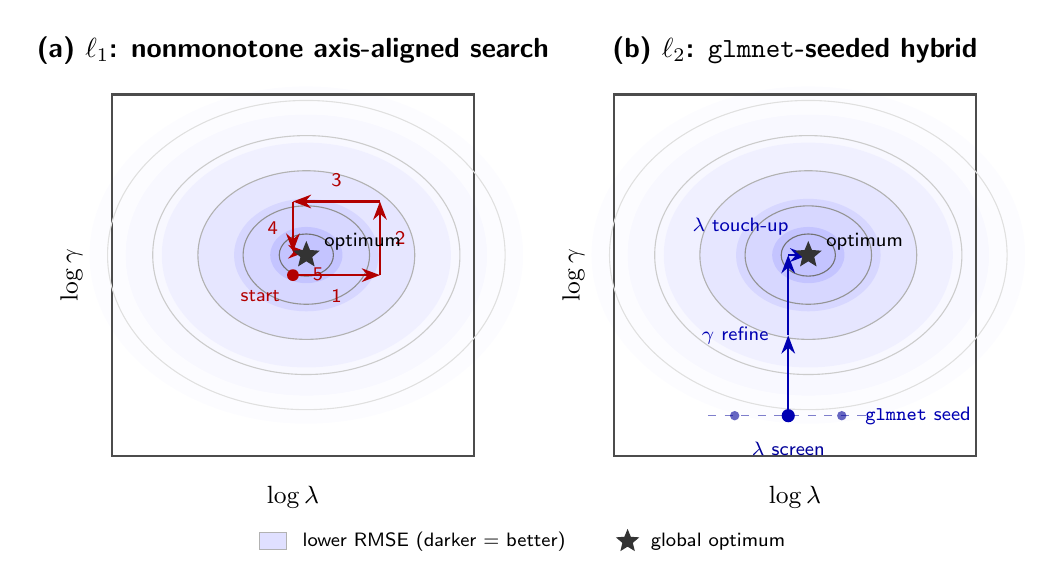
\begin{tikzpicture}[
  >=Stealth,
  scale=0.85,
  every node/.style={font=\small},
  searcharrow/.style={thick, ->, >=Stealth},
  contourline/.style={thin},
  boxframe/.style={thick, black!70},
]

%%% Panel (a): l1 branch — axis-aligned direct search %%%
\begin{scope}
  % Contour fills (outer to inner, darker = lower RMSE)
  \foreach \s/\f in {2.4/4, 2.0/8, 1.6/14, 1.2/22, 0.8/32, 0.4/45} {
    \fill[blue!\f!white, opacity=0.25] (2.9,3.0) ellipse ({\s*1.35} and {\s*1.05});
  }
  % Search box boundary
  \draw[boxframe] (0,0) rectangle (5.4,5.4);
  % Contour lines
  \foreach \s/\o in {2.2/12, 1.7/20, 1.2/30, 0.7/42, 0.3/55} {
    \draw[contourline, black!\o] (2.9,3.0) ellipse ({\s*1.35} and {\s*1.05});
  }
  % Axis labels
  \node[below] at (2.7,-0.3) {$\log\lambda$};
  \node[rotate=90, above] at (-0.3,2.7) {$\log\gamma$};

  % --- Search path: staircase from center ---
  \coordinate (a0) at (2.7,2.7);   % box center
  \coordinate (a1) at (4.0,2.7);   % probe lambda +
  \coordinate (a2) at (4.0,3.8);   % probe gamma +
  \coordinate (a3) at (2.7,3.8);   % shrink, probe lambda -
  \coordinate (a4) at (2.7,3.05);  % probe gamma -
  \coordinate (a5) at (2.9,3.05);  % small final step

  \draw[searcharrow, red!70!black] (a0) -- (a1);
  \draw[searcharrow, red!70!black] (a1) -- (a2);
  \draw[searcharrow, red!70!black] (a2) -- (a3);
  \draw[searcharrow, red!70!black] (a3) -- (a4);
  \draw[searcharrow, red!70!black] (a4) -- (a5);

  % Step labels (placed away from crowded center)
  \node[below, font=\scriptsize, red!70!black] at (3.35,2.62) {\textsf{1}};
  \node[right, font=\scriptsize, red!70!black] at (4.08,3.25) {\textsf{2}};
  \node[above, font=\scriptsize, red!70!black] at (3.35,3.88) {\textsf{3}};
  \node[left,  font=\scriptsize, red!70!black] at (2.62,3.4) {\textsf{4}};
  \node[below right, font=\scriptsize, red!70!black] at (2.85,2.95) {\textsf{5}};

  % Start marker
  \fill[red!70!black] (a0) circle (2.5pt);
  \node[below left, font=\scriptsize\sffamily, red!70!black] at (2.65,2.62) {start};

  % Optimum
  \node[star, star points=5, star point ratio=2.25, fill=black!80, inner sep=1.6pt] at (2.9,3.0) {};
  \node[right, font=\scriptsize\sffamily, xshift=3pt] at (2.9,3.2) {optimum};

  % Panel title
  \node[font=\normalsize\bfseries\sffamily, anchor=south] at (2.7,5.7)
    {(a) $\ell_1$: nonmonotone axis-aligned search};
\end{scope}

%%% Panel (b): l2 branch — glmnet-seeded hybrid %%%
\begin{scope}[shift={(7.5,0)}]
  % Contour fills
  \foreach \s/\f in {2.4/4, 2.0/8, 1.6/14, 1.2/22, 0.8/32, 0.4/45} {
    \fill[blue!\f!white, opacity=0.25] (2.9,3.0) ellipse ({\s*1.35} and {\s*1.05});
  }
  % Search box boundary
  \draw[boxframe] (0,0) rectangle (5.4,5.4);
  % Contour lines
  \foreach \s/\o in {2.2/12, 1.7/20, 1.2/30, 0.7/42, 0.3/55} {
    \draw[contourline, black!\o] (2.9,3.0) ellipse ({\s*1.35} and {\s*1.05});
  }
  % Axis labels
  \node[below] at (2.7,-0.3) {$\log\lambda$};
  \node[rotate=90, above] at (-0.3,2.7) {$\log\gamma$};

  % --- Lambda screening at low gamma ---
  \fill[blue!60!black, opacity=0.6] (1.8,0.6) circle (2pt);
  \fill[blue!60!black, opacity=0.6] (2.6,0.6) circle (2pt);
  \fill[blue!60!black, opacity=0.6] (3.4,0.6) circle (2pt);
  \draw[blue!60!black, dashed, opacity=0.5] (1.4,0.6) -- (3.8,0.6);
  \node[below, font=\scriptsize\sffamily, blue!60!black] at (2.6,0.35) {$\lambda$ screen};

  % Best screened + glmnet seed
  \fill[blue!70!black] (2.6,0.6) circle (2.8pt);
  \node[right, font=\scriptsize\sffamily, blue!70!black, xshift=5pt] at (3.4,0.6) {\texttt{glmnet} seed};

  % --- Gamma refinement (vertical) ---
  \draw[searcharrow, blue!70!black] (2.6,0.6) -- (2.6,1.8);
  \draw[searcharrow, blue!70!black] (2.6,1.8) -- (2.6,3.0);
  \node[left, font=\scriptsize\sffamily, blue!70!black] at (2.45,1.8) {$\gamma$ refine};

  % --- Local lambda touch-up (horizontal) ---
  \draw[searcharrow, blue!70!black] (2.6,3.0) -- (2.9,3.0);
  \node[above left, font=\scriptsize\sffamily, blue!70!black] at (2.75,3.15) {$\lambda$ touch-up};

  % Optimum
  \node[star, star points=5, star point ratio=2.25, fill=black!80, inner sep=1.6pt] at (2.9,3.0) {};
  \node[right, font=\scriptsize\sffamily, xshift=3pt] at (2.9,3.2) {optimum};

  % Panel title
  \node[font=\normalsize\bfseries\sffamily, anchor=south] at (2.7,5.7)
    {(b) $\ell_2$: \texttt{glmnet}-seeded hybrid};
\end{scope}

%%% Shared legend %%%
\begin{scope}[shift={(2.2,-1.4)}]
  \fill[blue!30!white, opacity=0.4] (0,0) rectangle (0.4,0.25);
  \draw[thin, black!30] (0,0) rectangle (0.4,0.25);
  \node[right, font=\scriptsize\sffamily] at (0.5,0.125) {lower RMSE (darker = better)};
  \node[star, star points=5, star point ratio=2.25, fill=black!80, inner sep=1.4pt] at (5.5,0.125) {};
  \node[right, font=\scriptsize\sffamily] at (5.7,0.125) {global optimum};
\end{scope}

\end{tikzpicture}
\caption{Search trajectories of \method{} on a stylized validation surface in $(\log\lambda,\log\gamma)$ space. Contour lines represent cross-validation RMSE levels; darker shading indicates lower (better) values. (a)~The $\ell_1$ branch starts at the box center and navigates via axis-aligned coordinate moves with nonmonotone acceptance. (b)~The $\ell_2$ branch starts from a \texttt{glmnet}-derived $\lambda$ seed, screens a small set of $\lambda$ candidates at low $\gamma$, refines $\gamma$ vertically, and adjusts $\lambda$ only when justified.}
\label{fig:concept}
\end{figure*}

\subsection{Efficiency metric}
Raw test RMSE, elapsed time, and validation-evaluation count are all useful, but none alone captures the intended trade-off. We therefore summarize many comparisons with a normalized gain-per-second score. For method \(m\) on dataset or regime \(d\), let \(r_{m,d}\) denote test RMSE, let \(r_{\mathrm{feat},d}\) be the featureless baseline RMSE, and let \(r_{\star,d}\) be the best RMSE achieved by any compared method on that dataset or regime. The normalized gain is
\begin{equation}
G_{m,d} =
\max\!\left(
0,
\min\!\left(
1,
\frac{r_{\mathrm{feat},d} - r_{m,d}}{r_{\mathrm{feat},d} - r_{\star,d}}
\right)
\right),
\label{eq:normalized_gain}
\end{equation}
and the efficiency summary is
\begin{equation}
\mathrm{GPS}_{m,d} = \frac{G_{m,d}}{t_{m,d}},
\label{eq:gain_per_second}
\end{equation}
where \(t_{m,d}\) is elapsed time in seconds. Higher values are better. If no method improves over the featureless baseline on dataset \(d\), we set \(G_{m,d}=0\) for all methods on that dataset. This score avoids rewarding the featureless model for being cheap while still penalizing methods that achieve little predictive gain.

\section{Experimental Design}\label{sec:design}
Throughout this section, ``retained'' refers to the final set of methods, datasets, and regimes kept for the main-text comparisons after preliminary screening excluded methods that were either redundant or consistently dominated. The supplementary baselines excluded from the retained panel are reported only in the appendix.

\subsection{Method panel}
The main paper uses a fixed retained panel: \texttt{featureless}, \texttt{grid}, \texttt{random}, \texttt{hooke\_jeeves}, \texttt{lbfgsb\_multistart}, \texttt{glmnet\_seeded}, and \codeid. The \texttt{featureless} model provides a null reference. Grid and random search represent exhaustive and stochastic black-box search, with random search motivated by the broader hyperparameter-optimization literature \cite{bergstra2012random}. Hooke--Jeeves and L-BFGS-B represent classical derivative-free and gradient-based baselines \cite{hooke1961direct,byrd1995lbfgsb,zhu1997lbfgsb}. \texttt{glmnet}-seeded search is the strongest structure-exploiting baseline for the current code base because the \(\ell_2\) implementation is itself built around a \texttt{glmnet} path \cite{friedman2010glmnet}. Extra synthetic baselines such as \texttt{bayesian\_opt} are reported only in the appendix, where they are interpreted as generic global-search comparators rather than direct methodological rivals \cite{jones1998ego,snoek2012practicalbo}.

\subsection{Real-data suites}
The retained \(\ell_1\) suite contains nine real datasets and compares \codeid{} against \texttt{glmnet\_seeded}. The retained \(\ell_2\) suite uses the same nine datasets with the full retained method panel. We report test RMSE, elapsed time, and validation-evaluation count from the aggregated summaries in the repository. For the \(\ell_1\) suite, the key operational comparison is \codeid{} versus \texttt{glmnet\_seeded}; for the \(\ell_2\) suite, we report both that head-to-head and the broader baseline context.

\subsection{Synthetic regime benchmark}
The synthetic benchmark contains \(30\) realized regimes across three families: \texttt{fusion\_helpful\_chain}, \texttt{heavy\_tailed\_outlier}, and \texttt{sparse\_shared\_noisy}. The benchmark is valuable because it separates regimes where fusion should be useful from regimes where the search problem is more adversarial. For \(\ell_2\), all \(30\) regimes completed under the updated benchmark after rerunning the two hardest sparse-noisy cases with a higher timeout.

\subsection{Surface diagnostics}
To make the search problem tangible, we include two \(\ell_2\) validation-surface diagnostics. The \texttt{school\_ilea} surface is useful because it prefers very small fusion. The \texttt{beijing\_air\_quality} surface is useful because it prefers substantial fusion and an interior optimum once the search range is widened. Together they show that \(\gamma\) is neither universally negligible nor universally dominant in the same direction.

\section{Results}\label{sec:results}
\subsection{Method roles}
Table~\ref{tab:methods} summarizes the retained comparison panel and the budget rationale.

\begin{table}[t]
\caption{Retained method panel and roles.}
\label{tab:methods}
\centering
\scriptsize
\begin{tabular}{>{\raggedright\arraybackslash}p{0.34\columnwidth}>{\raggedright\arraybackslash}p{0.51\columnwidth}}
\toprule
Method & Role in the comparison \\
\midrule
\texttt{featureless} & Null baseline with no tuning cost. \\
\texttt{grid} & Exhaustive reference over the search box. \\
\texttt{random} & Stochastic black-box baseline. \\
\texttt{hooke\_jeeves} & Classical derivative-free local search. \\
\texttt{lbfgsb\_}\\\texttt{multistart} & Gradient-based bound-constrained baseline. \\
\texttt{glmnet\_seeded} & Structure-exploiting warm-start baseline. \\
\codeid & Proposed low-budget solver-aware tuner. \\
\bottomrule
\end{tabular}
\end{table}

\subsection{Real-data \texorpdfstring{\(\ell_1\)}{L1} results}
The \(\ell_1\) results are the cleanest part of the paper. Across the nine retained real datasets, \codeid{} is faster than \texttt{glmnet\_seeded} on all nine datasets, uses less memory on seven, and achieves test RMSE no worse than the baseline on seven. Five datasets are triple-dominance cases in which \codeid{} is faster, lighter, and at least as accurate. The mean elapsed time drops from \(6.53\) seconds for \texttt{glmnet\_seeded} to \(3.25\) seconds for \codeid{}.

Table~\ref{tab:real_l1} shows the dataset-level pattern. The RMSE differences are usually tiny, but the time savings are systematic. The strongest wins appear on \texttt{rdatasets\_dietox}, \texttt{world\_bank\_wdi}, and \texttt{beijing\_air\_quality}. The only clear counterexample on accuracy is \texttt{rdatasets\_grunfeld}, where \texttt{glmnet\_seeded} attains a slightly lower test RMSE.

\begin{table*}[t]
\caption{Real-data \(\ell_1\) comparison between \texttt{glmnet\_seeded} and \codeid. Speedup is relative to \texttt{glmnet\_seeded}.}
\label{tab:real_l1}
\centering
\footnotesize
\begin{tabular}{lrrrrr}
\toprule
Dataset & RMSE (\texttt{glmnet}) & RMSE (\codeid) & Time (\texttt{glmnet}) & Time (\codeid) & Speedup \\
\midrule
Beijing Air Quality & 52.255 & 52.184 & 2.867 & 0.889 & 3.22 \\
Communities and Crime & 0.192 & 0.191 & 23.663 & 14.898 & 1.59 \\
King County House Sales & 389453.206 & 389453.206 & 8.957 & 3.071 & 2.92 \\
OWID CO\(_2\) & 8.043 & 8.043 & 0.220 & 0.062 & 3.55 \\
Radon Minnesota & 0.791 & 0.791 & 6.132 & 4.020 & 1.53 \\
RDatasets Dietox & 13.853 & 13.845 & 7.600 & 1.522 & 4.99 \\
RDatasets Grunfeld & 52.886 & 53.029 & 1.884 & 0.652 & 2.89 \\
School ILEA & 6.325 & 6.325 & 7.227 & 4.089 & 1.77 \\
World Bank WDI & 9682.956 & 9682.956 & 0.250 & 0.061 & 4.10 \\
\bottomrule
\end{tabular}
\end{table*}

\subsection{Real-data \texorpdfstring{\(\ell_2\)}{L2} results}
The \(\ell_2\) story is more nuanced. The redesigned \codeid{} is not the raw-RMSE winner on average across the full method panel, but it is now a credible efficiency method. Relative to \texttt{glmnet\_seeded}, it is faster on eight of nine datasets, lower in memory on seven, and no worse in RMSE on six. Mean elapsed time drops from \(1.585\) seconds to \(1.059\) seconds, while mean test RMSE is essentially tied at \(18389.207\) for \texttt{glmnet\_seeded} and \(18389.201\) for \codeid.

The strongest \(\ell_2\) gains for \codeid{} occur on \texttt{communities\_crime}, \texttt{king\_county\_house\_sales}, and \texttt{rdatasets\_dietox}. The main caveat is that raw gain-per-second can still favor \texttt{lbfgsb\_multistart} because it is extremely cheap; however, that method achieves RMSE no worse than \texttt{glmnet\_seeded} on only four of nine datasets, which makes it a less reliable practical choice. Figure~\ref{fig:real_efficiency} summarizes the head-to-head comparison between \codeid{} and \texttt{glmnet\_seeded}.

\begin{table*}[t]
\caption{Real-data \(\ell_2\) results. The best RMSE method is reported over the retained method panel.}
\label{tab:real_l2}
\centering
\footnotesize
\resizebox{\textwidth}{!}{%
\begin{tabular}{lrlrrrr}
\toprule
Dataset & Best method & Best RMSE & RMSE (\texttt{glmnet}) & RMSE (\codeid) & Time (\texttt{glmnet}) & Time (\codeid) \\
\midrule
Beijing Air Quality & \texttt{grid} & 34.3362 & 34.3375 & 34.3377 & 0.337 & 0.210 \\
Communities and Crime & \texttt{grid} & 0.1320 & 0.1398 & 0.1374 & 10.551 & 7.500 \\
King County House Sales & \texttt{lbfgsb\_multistart} & 164497.954 & 164498.531 & 164498.531 & 1.964 & 0.694 \\
OWID CO\(_2\) & \texttt{hooke\_jeeves} & 0.5392 & 0.5416 & 0.5401 & 0.238 & 0.157 \\
Radon Minnesota & \texttt{hooke\_jeeves} & 0.7210 & 0.7519 & 0.7433 & 0.222 & 0.187 \\
RDatasets Dietox & \codeid & 3.4793 & 3.5210 & 3.4793 & 0.206 & 0.272 \\
RDatasets Grunfeld & \texttt{lbfgsb\_multistart} & 48.9341 & 48.9364 & 48.9364 & 0.172 & 0.146 \\
School ILEA & \texttt{glmnet\_seeded} & 6.2878 & 6.2878 & 6.2890 & 0.380 & 0.231 \\
World Bank WDI & \texttt{hooke\_jeeves} & 909.720 & 909.818 & 909.818 & 0.196 & 0.132 \\
\bottomrule
\end{tabular}
}
\end{table*}

\begin{figure*}[t]
\centering

\includegraphics[width=0.93\textwidth]{../../figures/real_efficiency_compare.png}
\caption{Real-data comparison between \codeid{} and \texttt{glmnet\_seeded}. Each point is a dataset. Values to the right of the vertical line indicate that \codeid{} is faster; values below the horizontal line indicate that \codeid{} attains lower test RMSE. The \(\ell_1\) panel shows a clear practical win for \codeid. The \(\ell_2\) panel is more mixed on RMSE, but still strongly favors \codeid{} on elapsed time.}
\label{fig:real_efficiency}
\end{figure*}

\subsection{Synthetic results}
The synthetic benchmark clarifies when \codeid{} helps and when it mainly trades accuracy for budget. For \(\ell_1\), \codeid{} is the top efficiency method by normalized gain per second and is especially strong in the \texttt{fusion\_helpful\_chain} family, where it achieves the best mean RMSE among the retained methods and the lowest time among the serious competitors. In \texttt{heavy\_tailed\_outlier}, \texttt{lbfgsb\_multistart} attains the lowest mean RMSE, but \codeid{} remains comparably cheap. In \texttt{sparse\_shared\_noisy}, \texttt{glmnet\_seeded} has a small RMSE edge, whereas \codeid{} retains a clear time advantage.

For \(\ell_2\), the redesigned \codeid{} changes the story materially. The earlier implementation over-searched the validation surface and was too expensive to justify. After replacing the coarse two-dimensional search with the current \texttt{glmnet}-seeded hybrid, mean gain per second rises to \(2.52\), the highest among the synthetic \(\ell_2\) methods. That does not make \codeid{} the accuracy winner: \texttt{hooke\_jeeves} still has the lowest mean RMSE across the completed benchmark, and \texttt{grid} remains strong in difficult sparse-noisy regimes. The redesign instead turns \codeid{} into a credible low-budget method.

Table~\ref{tab:synth_summary} highlights the family-level picture, and Figure~\ref{fig:synth_family} summarizes the gain-per-second ranking across families.

\begin{table*}[t]
\caption{Synthetic family summary using retained baselines only. The ``best retained baseline'' column excludes \texttt{bayesian\_opt}, which is reported in the appendix.}
\label{tab:synth_summary}
\centering
\footnotesize
\resizebox{\textwidth}{!}{%
\begin{tabular}{lllrlll}
\toprule
Solver & Family & Best retained baseline & Baseline RMSE & Baseline time & \codeid{} RMSE & \codeid{} time / evals \\
\midrule
\(\ell_1\) & Fusion-helpful chain & \texttt{glmnet\_seeded} & 0.7059 & 1.907 & 0.7055 & 0.836 / 8.1 \\
\(\ell_1\) & Heavy-tailed outlier & \texttt{lbfgsb\_multistart} & 1.8031 & 9.116 & 1.8216 & 8.926 / 9.5 \\
\(\ell_1\) & Sparse shared noisy & \texttt{glmnet\_seeded} & 1.2707 & 36.641 & 1.2784 & 22.202 / 14.2 \\
\(\ell_2\) & Fusion-helpful chain & \texttt{hooke\_jeeves} & 0.6072 & 0.805 & 0.6061 & 0.323 / 10.1 \\
\(\ell_2\) & Heavy-tailed outlier & \texttt{hooke\_jeeves} & 1.2052 & 4.104 & 1.2297 & 1.925 / 9.2 \\
\(\ell_2\) & Sparse shared noisy & \texttt{hooke\_jeeves} & 1.1280 & 11.097 & 1.2005 & 2.929 / 8.8 \\
\bottomrule
\end{tabular}
}
\end{table*}

\begin{figure*}[t]
\centering

\includegraphics[width=0.98\textwidth]{../../figures/synthetic_family_gain.png}
\caption{Synthetic family comparison by normalized gain per second. The \(\ell_1\) panels show a clear efficiency advantage for \codeid. The redesigned \(\ell_2\) panels show the same pattern in \texttt{fusion\_helpful\_chain} and a strong cost-quality compromise in the other two families.}
\label{fig:synth_family}
\end{figure*}

\subsection{Surface diagnostics}
The surface diagnostics explain why a single search policy was not ideal for both solvers. Figure~\ref{fig:surface_diag} shows train and validation marginals for \(\texttt{school\_ilea}, \ell_2\) and \(\texttt{beijing\_air\_quality}, \ell_2\). In \texttt{school\_ilea}, the preferred \(\gamma\) region is near the lower edge, which is consistent with the broader observation that fusion can be neutral or slightly harmful there. In \texttt{beijing\_air\_quality}, the preferred \(\gamma\) region is clearly interior and substantially away from zero once the search range is widened. The two plots therefore support the same practical conclusion: the validation landscape is highly dataset-dependent, and the tuner needs to be prepared both for near-zero fusion and for clearly nontrivial fusion.

\begin{figure*}[t]
\centering
\begin{subfigure}[t]{0.48\textwidth}
  \centering
  
\includegraphics[width=\textwidth]{../../figures/school_ilea_l2_marginals.png}
  \caption{\texttt{school\_ilea}, \(\ell_2\)}
\end{subfigure}
\hfill
\begin{subfigure}[t]{0.48\textwidth}
  \centering
  
\includegraphics[width=\textwidth]{../../figures/beijing_air_quality_l2_marginals.png}
  \caption{\texttt{beijing\_air\_quality}, \(\ell_2\)}
\end{subfigure}
\caption{\(\ell_2\) validation-surface diagnostics for two representative datasets. (a)~shows per-fold marginals together with their across-fold means; (b)~shows single-fold marginals. In both cases the preferred regularization regime is not stable across datasets: \texttt{school\_ilea} pushes the optimum toward very weak fusion, while \texttt{beijing\_air\_quality} favors a clearly positive fusion level.}
\label{fig:surface_diag}
\end{figure*}

\section{Discussion}\label{sec:discussion}
Three practical conclusions follow from the experiments. First, \(\ell_1\) tuning is where \codeid{} is strongest. The method is consistently faster than the warm-start baseline and usually indistinguishable from it in test RMSE. Second, \(\ell_2\) tuning benefits from a different outer-search policy. The original \(\ell_2\) branch of \codeid{} spent too much budget on coarse two-dimensional exploration; the redesigned branch works better precisely because it borrows a \texttt{glmnet} seed and spends most of its budget screening \(\gamma\) quickly. Third, the validation landscape is not universally smooth or universally hostile. It changes with the solver and with the data regime. That is why a single generic tuning rule was a poor fit in practice.

The role of \texttt{lbfgsb\_multistart} deserves separate comment. On both real and synthetic \(\ell_2\) benchmarks it can appear very efficient because it is cheap, and on real \(\ell_2\) it attains the highest raw mean gain-per-second score. Yet its accuracy is not reliably competitive: in the real \(\ell_2\) retained suite it is no worse than \texttt{glmnet\_seeded} on only four of nine datasets. We therefore view it as a useful stress-test baseline rather than the preferred practical choice.

In that sense, \method{} is a conservative contribution. It does not attempt to replace established optimization theory. It offers an implementation-level answer to a recurring empirical problem: when fused-regression tuning is expensive, a small solver-aware search policy can outperform exhaustive tuning in wall-clock cost while retaining nearly all of the predictive performance.

\section{Conclusion}
We have presented \method{}, a solver-aware low-budget hyperparameter tuner for fused regression. The method is deliberately modest: it does not introduce new optimization theory, but rather shows that a small, solver-specific search policy can systematically reduce tuning cost while retaining nearly all of the predictive performance of more expensive alternatives. On the \(\ell_1\) side, the gains are clear and consistent; on the \(\ell_2\) side, the redesigned hybrid branch offers a credible efficiency--accuracy compromise. We hope the accompanying benchmark and efficiency metric encourage further work on practical tuning strategies for structured regularization problems.

\section{Limitations}
The paper has four important limitations. First, the evidence is empirical and does not establish convergence guarantees for \codeid. Second, the retained real-data suites are large enough to be informative, but still limited to nine datasets per solver. Third, the \(\ell_2\) results are stronger on efficiency than on raw accuracy, so the method should not be marketed as the universally best \(\ell_2\) tuner. Fourth, the exact solver behavior is tied to this code base, including the current \texttt{glmnet}-based \(\ell_2\) implementation and the repository's fused \(\ell_1\) solvers. A different fused-regression implementation could lead to different tuning surfaces and therefore different outer-search behavior.

\bmhead{Acknowledgements}
Not applicable.

\section*{Declarations}
\textbf{Funding} Not applicable.

\textbf{Conflict of interest/Competing interests} The authors declare no competing interests.

\textbf{Ethics approval and consent to participate} Not applicable.

\textbf{Consent for publication} Not applicable.

\textbf{Data availability} The real-data benchmark inputs are stored as processed grouped-regression files in the accompanying repository at \url{https://github.com/EngineerDanny/sparsefusion}. The synthetic benchmark inputs are generated from the regime manifests included in the repository.

\textbf{Materials availability} Not applicable.

\textbf{Code availability} All code used to fit the models, run the tuning benchmarks, and generate the manuscript figures is contained in the accompanying repository. The primary tuning implementation is in \texttt{local\_tune\_lambda\_gamma\_experiment\_round3.R}, and the manuscript figures are generated by \texttt{make\_paper\_figures.R}.

\textbf{Author contribution} Placeholder text. Author names and contributions will be finalized before submission.

\clearpage
\begin{appendices}

\section{Supplementary synthetic baselines}
Table~\ref{tab:appendix_synth_overall} reports the overall synthetic benchmark summaries including \texttt{bayesian\_opt}. These numbers are omitted from the main text to keep the main comparison aligned with the retained real-data method panel.

\begin{table*}[ht]
\caption{Overall synthetic benchmark summaries including \texttt{bayesian\_opt}.}
\label{tab:appendix_synth_overall}
\centering
\footnotesize
\begin{tabular}{llrrr}
\toprule
Solver & Method & Time (s) & Test RMSE & CV evals \\
\midrule
\(\ell_1\) & \texttt{featureless} & 0.004 & 4.236 & 0.0 \\
\(\ell_1\) & \texttt{lbfgsb\_multistart} & 8.955 & 1.350 & 9.2 \\
\(\ell_1\) & \codeid & 10.655 & 1.269 & 10.6 \\
\(\ell_1\) & \texttt{glmnet\_seeded} & 19.971 & 1.270 & 20.7 \\
\(\ell_1\) & \texttt{hooke\_jeeves} & 20.356 & 1.271 & 20.8 \\
\(\ell_1\) & \texttt{bayesian\_opt} & 20.483 & 1.265 & 20.6 \\
\(\ell_1\) & \texttt{random} & 34.766 & 1.291 & 36.0 \\
\(\ell_1\) & \texttt{grid} & 34.940 & 1.268 & 36.0 \\
\midrule
\(\ell_2\) & \texttt{featureless} & 0.005 & 4.236 & 0.0 \\
\(\ell_2\) & \codeid & 1.725 & 1.012 & 9.4 \\
\(\ell_2\) & \texttt{glmnet\_seeded} & 2.142 & 1.058 & 20.1 \\
\(\ell_2\) & \texttt{lbfgsb\_multistart} & 3.707 & 1.052 & 8.8 \\
\(\ell_2\) & \texttt{hooke\_jeeves} & 5.335 & 0.980 & 30.7 \\
\(\ell_2\) & \texttt{bayesian\_opt} & 11.873 & 0.997 & 28.2 \\
\(\ell_2\) & \texttt{grid} & 17.402 & 0.986 & 36.0 \\
\(\ell_2\) & \texttt{random} & 18.289 & 0.986 & 36.0 \\
\bottomrule
\end{tabular}
\end{table*}

\section{Why the \texorpdfstring{\(\ell_2\)}{L2} redesign mattered}
The original \(\ell_2\) branch of \codeid{} used a coarse two-dimensional search followed by local refinement. On the synthetic benchmark that design used more than \(50\) validation evaluations on average and spent enough time exploring weak directions that its low-budget claim was hard to defend. The current branch instead uses a \texttt{glmnet}-seeded \(\lambda\) anchor, a small \(\gamma\) screen, and a local \(\lambda\) adjustment only when screening indicates that the seed is not already adequate. On the completed synthetic \(\ell_2\) benchmark, this redesign reduces the average validation count to \(9.37\) while preserving competitive predictive performance. The main-text \(\ell_2\) results should be interpreted as evidence for that redesign, not as evidence that every direct-search variant would behave similarly.

\end{appendices}

{\sloppy\bibliography{sn-bibliography}}

\end{document}
